\section{Approach}
\label{s:approach}
%Approach; What selection of deep uncertainty methods are you using, in what order, and why? This should be clearly motivated and grounded in the literature

% Analysis is carried out across the explicated rival problem framings and relies on state-of- the-art deep uncertainty techniques

% Analysis is carried out across the explicated rival problem framings and relies on state-of- the-art deep uncertainty techniques
Multiple alternative approaches were considered to analyse the explicated problem framings. Ultimately, a straightforward combination of techniques were adopted to analyse and interpret the problem framings of Gorssel, as well as it's two rival/coalition-forming actors, Deventer and Overijssel. A multi-scenario multi objective robust decision making process was chosen for the analysis and selection of policy approaches. This approach was selected for the ability to achieve a balance between finding robust solutions that are locally optimal in individual scenarios, while also being computationally efficient, given constraints in time and computing power \parencite{bartholomew_considering_2020}. A flow diagram for this approach is shown in Figure \ref{fig:msmordm}.

\begin{figure}[h]
    \centering
    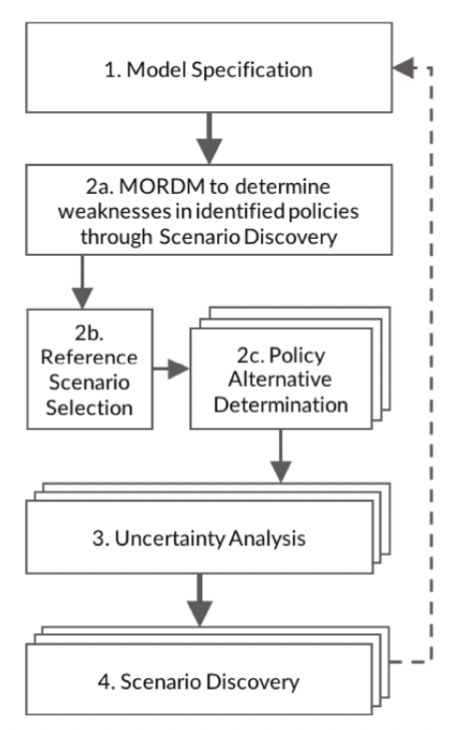
\includegraphics[width=0.5\textwidth]{report/figures/msmordm.png}
    \caption{The MSMORDM Process from \citeauthor{bartholomew_considering_2020}}
    \label{fig:msmordm}
\end{figure}

%In what order are we using the tools and why are we using them this way
\begin{enumerate}
    \item  Problem formulation for the three actors in the context of the model (the multiple objectives part of MSMORDM)\\
    \textbf{1a.} Trindade et al - Taking the value of the worst performing actor for each objective.
    \item  Generate 50,000 scenarios for each of the three actor problem formulations
    \item  Scenario discovery using the PRIM algorithm to find which uncertainties result in worst scenarios
    \item Scenario selection of worst case, best case, and 'middle-ground' case for testing of policies (the multi-scenario part of MSMORDM) (cite: Eker and Kwakkel)
    \item Robust decision making using robustness objectives (satisficing and regret-based) \textbf{(cite: McPhail)}
    \item Sensitivity analysis of 'robust' policies for the three actors.
    \item Identify where there are policies that are consistent (or at least similar) between actors to support coalition forming (in the case of consistent policies) or informing policy negotiations (in the case of inconsistent policies).
\end{enumerate}


%btw, we should mention in the report that since we've increased the number of uncertainties, we need to use more scenarios for a lot of stuff, lol